\section{Saffron}
\label{sec:saffron}

\begin{spice}\label{spice:saffron}
\textsc{Saffron} \hfill \href{https://powo.science.kew.org/taxon/436688-1}{POWO} \\
\textbf{English:} \textit{saffron}. 
\textbf{Arabic:} {\arabicfont{زعفران}} \textit{zaʿfarān}. 
\textbf{Chinese:} {\traditionalchinesefont{藏紅花}} \textit{zànghónghuā} [Tibetan-red-flower]; 西紅花 \textit{xīhónghuā} [western-red-flower]; 番紅花 \textit{fān​hóng​huā} [foreign-red-flower]. 
\textbf{Hungarian:} \textit{sáfrány}.  \\
\noindent{\color{black}\rule[0.5ex]{\linewidth}{.5pt}}
\begin{tabular}{@{}p{0.25\linewidth}@{}p{0.75\linewidth}@{}}
Plant species: & \taxonn{Crocus sativus}{L.} \\
Family: & \textit{Iridaceae} \\
part used: & stigma (style) \\
Region of origin: & Greece \\
Cultivated in: & Iran; Spain; Kashmir; etc. \\
Color: & deep red; dyes in orange \\
\end{tabular}
\end{spice}

\begin{figure}[!ht]
	\vspace{-4ex}
	\centering
	\subfloat[]{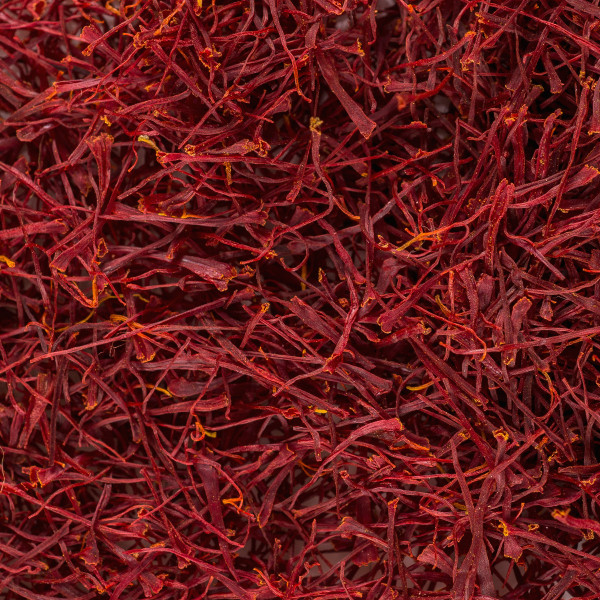
\includegraphics[width=0.3\linewidth]{imgs/spices/saffron-1.jpg}}
	\hfill
	\subfloat[]{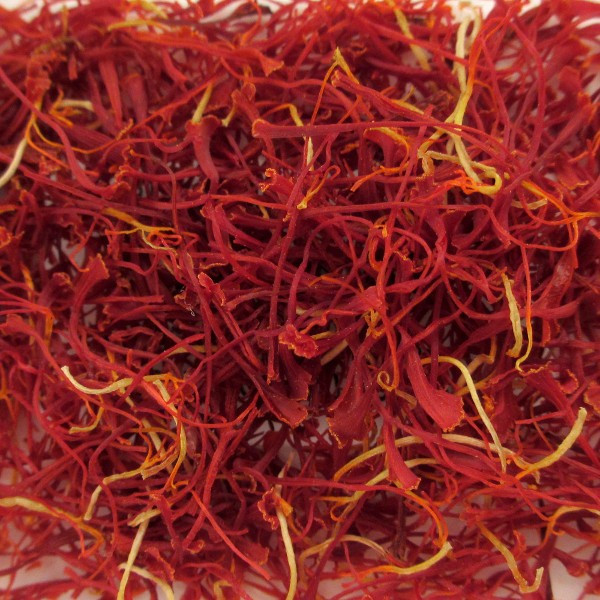
\includegraphics[width=0.3\linewidth]{imgs/spices/saffron-2.jpg}}
	\hfill
	\subfloat[]{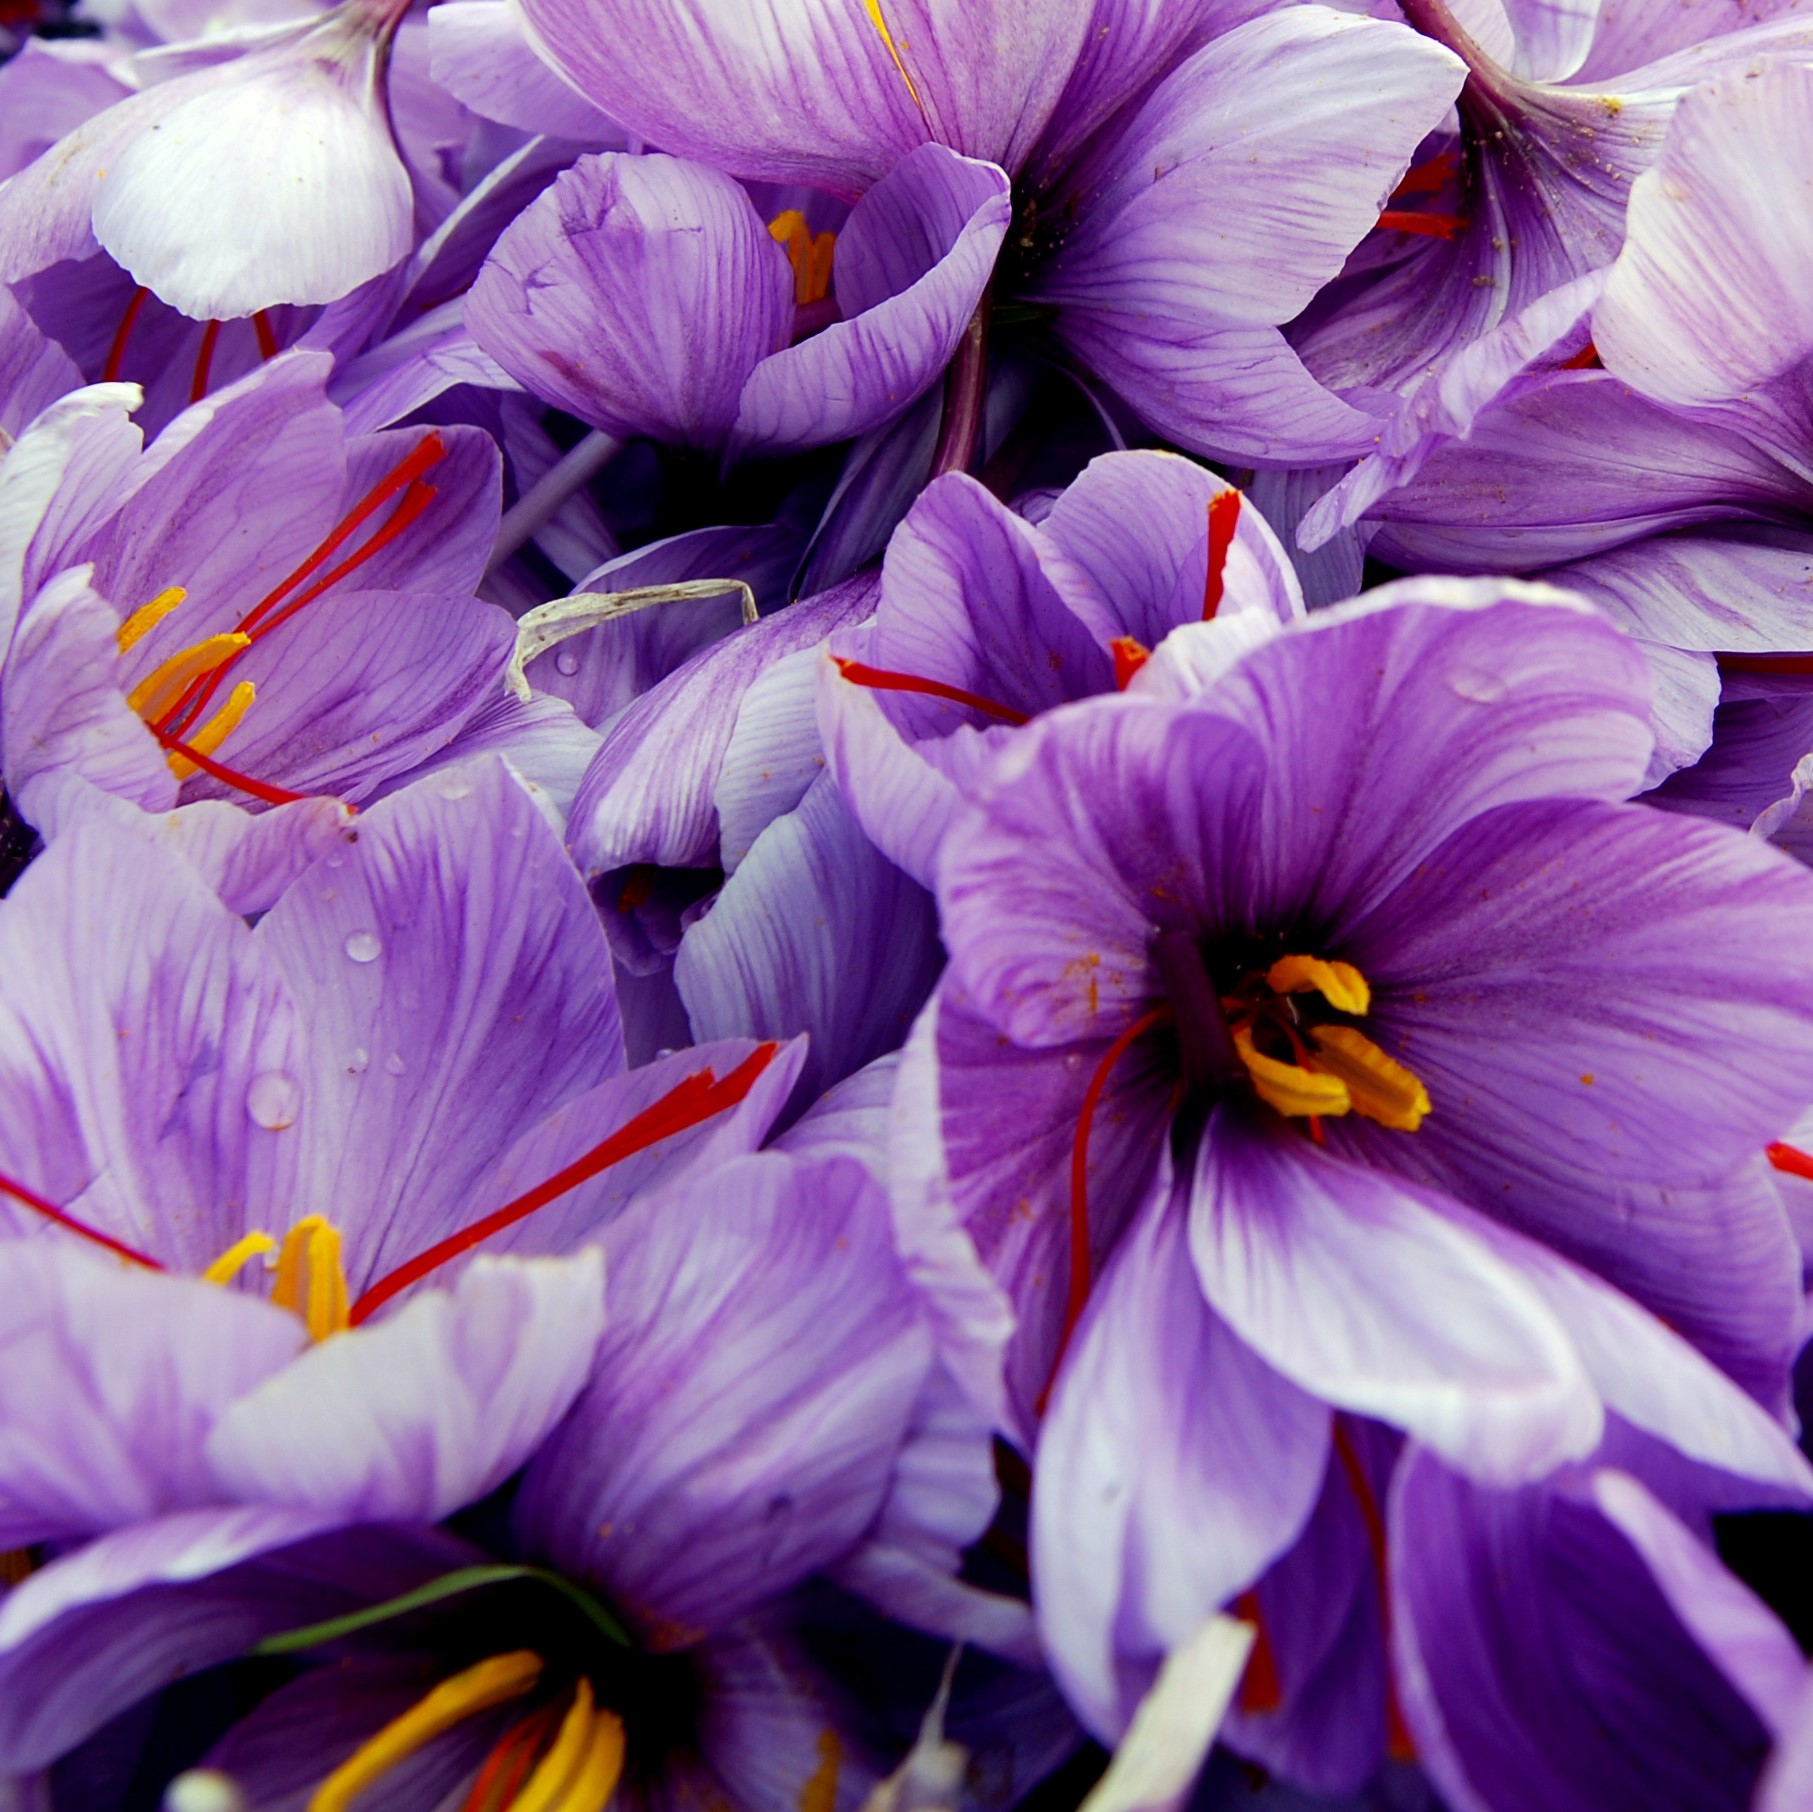
\includegraphics[width=0.3\linewidth]{imgs/spices/saffron-3.jpg}}
	\caption[Saffron threads and flowers]{Saffron threads from the Quercy region of France (a), from La Mancha, Spain (b), and saffron flowers from Khorasan, Iran (c). \textit{Crocus sativus}. Credits: Aromatiques (a, b); Vathlu (c)\protect\footnotemark}
	\label{fig:saffron_imgs}
\end{figure}

\footnotetext{Wikimedia Commons CC4.0 \url{https://commons.wikimedia.org/wiki/File:Saffron_Flowers_in_Khorasan,_Iran.jpg}}

Saffron is the dried, dark red stigmas (and styles) of the saffron crocus flower. It owes its reputation to its unique, fragrant aroma, vivid coloring properties, and the fact that it is the costliest spice by weight. Its high price is due to the labor-intensive harvest, and the large growing area it requires. Saffron has been cultivated for thousands of years now, and it is famous for being the most expensive spice throughout much of recorded history. Saffron is a medicine, dye, and spice, with important cultural roles. It gives flavor to Spanish paella, and lends the orange hue to Buddhist monks' robe. In Iran this ``red gold'' is the pinnacle of all spices, it is a ubiquitous ingredient of Persian cuisine and an important export product. It is cultivated in Mediterranean climate and semi-arid areas, including Spain, Morocco, Iran, Afghanistan, Kashmir, and more recently New Zealand.

% SAFFLOWER ETYMOLOGY
% The form has been influenced by association with the words saffron (French safran) and flower (Italian fiore, French fleur); although safflower is a wholly different plant from saffron, the former was often used as a substitute for the latter in medicine, whence the name bastard saffron.


% dye 
% style 
% civilization 
% gathered

% Mathew:
% Saffron has been well known as a dye and medicinal substance since very early times, indeed it was so important in the Middle Ages that a book of almost three hundred pages—Crocologia by Hertodt (Jena, 1671)—was published giving instructions for the treatment of the diseases using Saffron. Much earlier than this however it was mentioned as a perfume by Dioscorides (1st century A.D.) who gave an account of the prepara tion of saffron-scented lotions. It is also said to have been used in ancient times as a perfume in halls, courts and theatres, the flowers being strewn on the floors. As a dye it has been in use since early Greek times, although its use is now very restricted since it is not economically worthwhile to utilize land in this way. It has been calculated that the stigmas of over four thousand flowers are required to produce one ounce of dried saffron. As it therefore probably requires several acres of C. sativus to produce a few pounds of saffron it is hardly likely that it will continue for long as a crop, even in country communities such as at Safranbolu in Turkey where it is still cultivated. As a culinary flavouring and colouring agent it is still used to a small extent in various dishes and in baking since only relatively minute quantities are required compared to those needed in the processes of dyeing.—Medicinally it has been recommended by herbalists for almost any complaint, Hertodt claiming that it cured such diverse disorders as hernia and cerebral haemorrhage, while Rivenius, a 17th century physician, noted that a large dose of saffron given to a woman caused death after the third day, although this should not perhaps be classed as a medicinal pro perty. Apoplexy and "senseless" extravagant gaitey have also been listed as possible after effects
% The origin of the C. sativus clone which exists today is unknown but it is highly probable that it is the same as that grown in England in the fourteenth century. There is even the possibility that it was known as long ago as 1600 B.C. for at Knossos in Crete there exist designs on Minoan frescoes and pottery in which a Crocus with simple long-exserted red stigma branches is depicted. No Crocus exhibits this feature better than C. sativus although in some forms of C. cart wrightianus the branches are a little longer than the perianth segments. It is of course impossible to say whether the Minoans were cultivating the actual clone which still exists today, or a form of C. cartwrightianus, a species which occurs naturally on Crete. The argument is perhaps in favour of the latter case since some of the Crocus depicted are white flowered and this species has a marked tendency to produce albinos. Whichever case is true, it is apparent that the Minoans possessed plant which had exceptional better yield of saffron The most likely explanation sativus is that it was because of its apparent duction of the clone man throughout Europe examined from sources France are so uniform of being derived from very similar

\subsection{The Botany, Origins, and Cultivation of Saffron}

The bulbous plant species yielding the spice and dye is a sterile \gls{cultigen}\footnote{Coined in 1918 by Liberty Hyde Bailey (1858–1954) an American horticulturist and botanist, cultigen refers to a plant species that is a result of artificial selection or alteration, typically being cultivated by humans only, sustaining no wild individuals. \url{https://www.actahort.org/books/799/799_23.htm}} called \textit{Crocus sativus} L. \autocite[124]{van_wyk_culinary_2014}, \textit{sativus} meaning `cultivated' in Latin. Saffron does not grow in the wild, as it cannot survive without human handling/intervention \autocite[469]{peter_handbook_2012}. It relies entirely on horticulture, there are no known wild variants, and so the origins of this plant are not entirely clear. Although by now it has propagated throughout much of Europe and Western Asia, its proposed regions of origin range from the Eastern Mediterranean to Asia Minor (today's Greece, Turkey, Iran). After comparing the related taxa, it is now believed that it was developed in ancient Greece from a wild progenitor, most probably \textit{Crocus cartwrightianus} Herb.\footnote{POWO: \url{https://powo.science.kew.org/taxon/436500-1}}, which also bears the most resemblance to it \autocite{mathew_crocus_1977}. Growing in Greece -- Attica, the Cyclades, and Crete in the Aegean Sea, this species was likely selected for its long stigmas \autocite[248]{mabberley_mabberleys_2017}.




As a crop, saffron spread to various places around the globe, and so today there are some historically important saffron growing regions such as Iran, Kashmir, Spain. Iran is by far the top producer of saffron, accounting for two thirds of the global market (or up to 90\& in other sources), which is around 300 tons/year \autocite[248]{mabberley_mabberleys_2017}. Spain also produces superb quality saffron in a relatively small, protected designation of origin (PDO) area in La Mancha; their skill results with the highest yields per hectare, and they prepare around 47 tons per annum. Interestingly, Spain was also the top importer of saffron in the last decade. The race for the ``who has best saffron is the world'' is usually joined by India, as Kashmiri saffron is also held in high regard (saffron is only cultivated in the Jammu \& Kashmir territory of India). 

To produce one kilogram of saffron, one needs around a 100 000-250 000 flowers...



There are many other decorative flowering species native to Europe that look very similar to the saffron crocus, but they are not used as spice, take for example the toxic ``autumn crocus, meadow saffron, naked lady'' \textit{(Colchicum autumnale)}.







\subsubsection{Production, cultivation and harvest}

Being sterile, saffron croci has to be artificially propagated by dividing the corms (bulbs) during the summer dormant period, and harvested in autumn when they flower \autocite[124]{van_wyk_culinary_2014}. Work has to be fast and organised, because all the flowers blossom synchronously in a short, one or two week period, and they can be only gathered at dawn when they open; the flowers slowly wilt as the day passes. Each purple flower has three bright crimson stigmas that are connected to the plant's ovary in the stem by a yellow style, this is called a ``thread''. The saffron threads have to be carefully hand-picked from the harvested flowers, and the spice's quality depends on what part of the threads are then sold. The upper, vivid red stigmas have the most strong aroma, while the lower styles have almost none. Figure \ref{fig:saffron_grades} shows different quality saffron trims, with the popular terminology taken from Persian.

Rivaling with the price of gold, this fragrant spice is also known as ``red gold''. As of January 2022, a spice shop in Hong Kong is selling a 0.1 gram sample of saffron style\footnote{Style refers to a narrow, upward extension of the ovary in a flower, connecting it to the stigmatic papillae (\url{https://www.britannica.com/science/style-plant-anatomy})} for double the unit price as any other spice in their supply.\footnote{Source: \url{https://regencyspices.hk/collections/spices/products/saffron}}

showing which part of the thread is trim


\begin{figure}[!hbt]
    \centering
    \includegraphics[width=\linewidth]{imgs/saffron_grades.png}
    \caption{Different grades of saffron. From left to right: Daste (bunch saffron), Pushal, Negin, Super Negin, Sargol, Konj (white saffron)}
    \label{fig:saffron_grades}
\end{figure}






% In modern food processing, safflower
% (false saffron, sometimes fraudulently sold as true
% saffron), turmeric (Indian saffron) or artificial
% colours and flavours are mostly used.2

% (Arabic za’fran, 106 fls to give 10 kg
% dried spice) form. imp. dye (alpha crocin, crocetin – a carotenoid) in anc. Greece derived
% from stigmas, now largely prep. in Spain (5000 ha yielding 4.7 × 109 stigmas, 47 t spice
% per annum, world total 300 t, 100–170 t. from Iran, best from Kashmir) for cooking (bitter
% taste due to picrocrocin) & colouring foods esp. Spanish rice, bouillabaisse, while saffron
% cakes & loaves trad. in Cornwall, v. imp. constituent of Fernet-Branca (It. digestif;
% prod. alleged to consume 75% world’s saffron), 'karkom' (orig. of word crocus) of Song of
% Solomon, most prob. that featured onMinoan pottery & frescoes (1600 BC), used in c. 90
% med. conditions (steroids; but 2 g harmful), app. reducing arteriosclerosis poss. explaining
% low levels of cardiovascular disease in Spain where consumption is high (richest
% known source of vitamin B2), constituent of laudanum

% About
% 300 tons are produced each year1 – mainly in
% Iran and Spain but also Turkey, Greece, Italy and
% Kashmir (considered the best quality).1












% Saffron is a culturally very important spice, its roles go way beyond being just an aromatic flavoring. 

\subsubsection{The History of Saffron}

Depictions of saffron were found at the wall-paintings of Thera (modern Santorini), on the Aegean Sea. These frescoes are one of the few remaining artistic examples of the ancient Minoan culture, going back as early as the first half of the 2\textss{nd} millennium BC \autocite[29-31]{doumas_wall-paintings_1992}. The murals at the archaeological site of Akrotiri have been preserved in pyroclastic ash due to a massive volcanic eruption, somewhere around the last decades of the \nth{17} century BC, similar to Pompeii.



% \begin{figure}[!hbt]
%     \centering
%     \includegraphics[width=\linewidth]{imgs/saffron_gatherers.jpg}
%     \caption{Saffron-gatherers. Details from the mural on the east wall in room 3a, first floor, at Xeste 3 site, Akrotiri \autocite[152]{doumas_wall-paintings_1992}.}
%     \label{fig:saffron_gathererss}
% \end{figure}



\begin{figure}[!hbt]
    \centering
    \subfloat{\includegraphics[width=0.482\linewidth]{imgs/saffron_gatherers_l.jpg}}
    \hfill
    \subfloat{\includegraphics[width=0.482\linewidth]{imgs/saffron_gatherers_r.jpg}}
    \caption{Saffron-gatherers. Details from the mural on the east wall in room 3a, first floor, at Xeste 3 site, Akrotiri \autocite[152]{doumas_wall-paintings_1992}.}
    \label{fig:saffron_gatherers}
\end{figure}



% producers Iran....

% orange dye

% Legends



% folk etymology





% Wyk:
% 2 as a source of spice and orange-yellow
% dye.

% About
% 300 tons are produced each year1 – mainly in
% Iran and Spain but also Turkey, Greece, Italy and
% Kashmir (considered the best quality).1
% Harvesting The flowers open at dawn and are
% picked in the early morning before they wilt.
% The styles and stigmas are removed by hand and
% then dried. Harvesting and processing is a labourintensive
% activity that contributes to the high price
% of saffron. In modern food processing, safflower
% (false saffron, sometimes fraudulently sold as true
% saffron), turmeric (Indian saffron) or artificial
% colours and flavours are mostly used.2
% Culinary uses Saffron is famous as the essential
% ingredient of French bouillabaisse, Spanish paella
% and Italian risotto. It is an important spice in many
% traditional Mediterranean, Arabian and Indian rice
% and curry dishes, as well as semolina and milk
% puddings. As a reddish-yellow dye and flavourant,
% it is still much used in the production of butter,
% cheese, pastries, confectionery (e.g.,saffron cakes
% in Cornwall,1 saffron bread in Sweden), sauces and
% liqueurs (e.g.,chartreuse).
% Flavour compounds The compounds responsible
% for the unique colour, taste and aroma of saffron are
% all derived from carotenoids.3 The colour comes
% from crocin (and crocetin), while the bitter taste is
% due to a glucoside, picrocrocin.3 Several volatile
% compounds such as isophorone and especially safranal
% are responsible for the flavour and aroma,3–5
% often described as “hay-like”, or “seabreeze-like”.
% A minor compound, 2-hydroxy-4,4,6-trimethyl-
% 2,5-cyclohexadien-1-one is now considered to be
% the most powerful aroma constituent of saffron,
% followed by safranal.4,5
% Notes Saffron is the richest known source of
% vitamin B2. The maximum safe dose of saffron is
% 1 g (0.035 oz.) per day.

% Mabberley:
% C. sativus L. (saffron, a sterile autotriploid cultigen prob. selected for long stigmas from
% C. cartwrightianus Herb. (Greece)) – source of saffron (Arabic za’fran, 106 fls to give 10 kg
% dried spice) form. imp. dye (alpha crocin, crocetin – a carotenoid) in anc. Greece derived
% from stigmas, now largely prep. in Spain (5000 ha yielding 4.7 × 109 stigmas, 47 t spice
% per annum, world total 300 t, 100–170 t. from Iran, best from Kashmir) for cooking (bitter
% taste due to picrocrocin) \& colouring foods esp. Spanish rice, bouillabaisse, while saffron
% cakes \& loaves trad. in Cornwall, v. imp. constituent of Fernet-Branca (It. digestif;
% prod. alleged to consume 75\% world’s saffron), 'karkom' (orig. of word crocus) of Song of
% Solomon, most prob. that featured onMinoan pottery \& frescoes (1600 BC), used in c. 90
% med. conditions (steroids; but 2 g harmful), app. reducing arteriosclerosis poss. explaining
% low levels of cardiovascular disease in Spain where consumption is high (richest
% known source of vitamin B2), constituent of laudanum
% crocus, autumn Colchicum spp. esp. C. autumnale; Chilean c. Tecophilaea cyanocrocus; Dutch
% c. Crocus neapolitanus; saffron c. C. sativus

``Of no foreign product are the notions of the Chinese vaguer than
of saffron.'' Laufer

\subsection{The Names of Saffron}
\label{sec:names_of_saffron}

\subsubsection{English}

\begin{etymology}\label{ety:saffron}
\textbf{English} \textit{saffron}, ca. 1200; cf. Middle English \textit{saf(f)rǒun}
< \textbf{French} \textit{safran} `id.', c. 1150; cf. Middle Low German \textit{safferân}, Middle Dutch \textit{saffraen} (Dutch \textit{saffraan}), Middle High German \textit{saffrân} (modern German \textit{safran})
< \textbf{Medieval Latin} \textit{saffrānum} `id.'
< \textbf{Arabic} {زعفران} \textit{zaʿfarān} `id.', (not connected with \textit{ṣafrā'} feminine of \textit{aṣfar} `yellow'); cf. Turkish, Persian, and Hindi; Jewish Aramaic \textit{zaʿperānā}; Spanish \textit{azafran}, Portuguese \textit{açafrão}; the word without this prefix gives rise to Italian \textit{zafferano, zaffrone}, Provençal \textit{safran, safrá}, Catalan \textit{safrá}, French \textit{safran}, medieval Latin \textit{safranum}, medieval Greek ζαϕρᾶς \textit{zaforás}, modern Greek σαϕράνι \textit{safráni}, Russian \textit{šafran}. \footnote{\textcite[s.v. saffron]{oed}; \textcite[saf(f)rǒun]{med}; \textcite[s.v. safran]{tlfi}; \textcite{wehr_dictionary_1976}}
\end{etymology}

The word \textit{saffron}, referring to  bright red stigmas used as spice and dye was first attested in the start of the \nth{13} century. It entered Middle English via Old French \textit{safran}\footcite[safran \link{https://www.cnrtl.fr/etymologie/safran}]{tlfi}, a \nth{12} century word from Medieval Latin \textit{safrānum}, which is a loanword from Arabic \textit{zaʿfarān} .\footcites[saffron]{oed}[saf(f)rǒun]{med} The origin of the Arabic word is unknown, but it has been compared to Akkadian \textit{azupīru}.\footcite[saffron \link{https://www.ahdictionary.com/word/search.html?q=saffron}]{ahd} The meaning referring to the plant and flower saffron crocus (\textit{Crocus sativus}) is attested from the \nth{15} century onwards, which means that this is a case where the product was known before its plant source (just like in many other cases).

I must emphasize the importance of saffron's coloring properties. Even far away from its homeland in musty England, the word \textit{saffron} soon gained a meaning of `orange-yellow color', attested as early as the late \nth{14} century and appearing in literature as the color or robes: ``Your sonne was misled with a snipt taffata fellow there, whose villanous saffron wold haue made all the vnbak'd and dowy youth of a nation in his colour.'' (W. Shakespeare \textit{All's Well that Ends Well} (1623) iv. v. 2, \cite[saffron]{oed}) Furthermore, \textit{saffron} as a verb in the sense `to dye with saffron; to give a saffron-yellow color to' is attested from the end of the \nth{16} century. E.g.: ``In Ireland..they saffron all their wearing linnen.''\footcite[saffron, v.]{oed}

This is a good example for the kind of cultural acclimatization a spice can achieve that shines through language use: if the name of the spice becomes an adjective and even a verb, it must be reflecting on a situation that is marked by widespread---or at least fashionable---usage.

\begin{table}[!ht]
\centering
\begin{tabularx}{\textwidth}{@{}l>{\itshape \small}lL>{\small}l@{}}
\toprule
\textbf{\#} & \multicolumn{1}{l}{\textbf{Species}} & \multicolumn{1}{l}{\textbf{Name}} & \multicolumn{1}{l}{\textbf{Source}} \\
\midrule
\textbf{1}	& \textbf{Crocus sativus}	& \textbf{saffron}	& \textbf{\textcite{van_wyk_culinary_2014}} \\
\bottomrule
\end{tabularx}
\caption{Various names for saffron in English.}
\label{table:names_saffron_en}
\end{table}




Safflower

\subsubsection{Arabic}

\begin{etymology}\label{ety:zafaran}
\textbf{Arabic} {زعفران} \textit{zaʿfarān} `saffron', (not connected with ṣafrā' feminine of aṣfar yellow); cf. Turkish, Persian, and Hindi; Jewish Aramaic zaʿperānā; Spanish azafran, Portuguese açafrão; the word without this prefix gives rise to Italian zafferano, zaffrone, Provençal safran, safrá, Catalan safrá, French safran, medieval Latin safranum, medieval Greek ζαϕρᾶς, modern Greek σαϕράνι, Russian šafran. 
<\textss{?} \textbf{Pahlavi} \textit{zarparān} `saffron' [golden thread], \textit{zar} `gold' + \textit{par} `feather' + \textit{-ān} `pl.', a pseudo-etymological explanation
<\textss{?} \textbf{Akkadian} {\cu{𒌑𒄯𒊕}} \textit{azupīru, azupīrānu} `a spice and medicinal plant', (unlikely etymon)\footnote{\textcite{wehr_dictionary_1976}; \textcites[]{asbaghi_persische_1988}[65, 98]{mackenzie_concise_1986}[safran]{ns}; \textcites[33]{black_concise_2000}[vol. 2, 530-531]{roth_assyrian_2004}}
\end{etymology}

It can be often read \autocite[e.g., in][124]{van_wyk_culinary_2014} that the original Arabic word means `yellow', due to the conflation of Arabic \textit{ṣ-f-r} (the concept of yellow) with the word for saffron, but this is unfounded folk-etymologization and thus a false cognate; there is no known version with ṣ /sˤ/ in Arabic and there is no supporting evidence for a similar sound change.

% Contrary to a supposed Arabic version of ṣaˁfarān besides the usual zaˁfarān (NS, ``safran''), an Ottoman Turkish variation using ص is native to Turkish, due to the /z/ \rightarrow /s/ sound change in certain Turkish dialects or (obfuscated with) hyper-correction towards assumed, more conservative Arabic spelling.
% https://en.wiktionary.org/wiki/%D8%B2%D8%B9%D9%81%D8%B1%D8%A7%D9%86#Ottoman_Turkish
% https://en.wiktionary.org/wiki/z%C9%99ngin#Azerbaijani
% https://archive.org/details/in.ernet.dli.2015.105040/page/n118/mode/2up?view=theater

On the other hand, Arabic \textit{zaʿfarān} is an obvious candidate to be a loanword---no question about it---and it has been proposed by \textcite{asbaghi_persische_1988} that it might be coming from Middle Persian \textit{*zarparān}, meaning `gold thread', or 'golden feathers', as in \textit{zar} `gold' + \textit{par} `feather; wing; leaf' + \textit{-ān}, the historical marker for plurals in Persian \footcite[65,98]{mackenzie_concise_1986}, an explanation that found its way to other dictionaries\footcite[cf.][safran]{ns}. Unfortunately, this claim was made in a publication that was deemed to be ``unserious'' \autocite[9]{ullmann_zur_1997} and even a ``scandal'' \autocite[315]{niehoff_review_1989} by scholars in the field, and seem to be a classic case of folk etymologization from a Persian as a foreign language teacher. Nevertheless, it remains cited in many places. An even more obscure path takes us to Akkadian; the literature sometimes mentions \textit{azupīru} or \textit{azupīrānu}\footcite[33]{black_concise_2000} as a possible source, but the \gls{CAD} finds this unlikely, citing that the uses for this plant are inconsistent with that of saffron, for example the mentions of its seeds.\footcite[531]{roth_assyrian_2004} 
Nevertheless, the assumption that we could be dealing with a regional \gls{wanderwort} that can be attested in various Semitic languages is not wrong, and to tell the truth I was rather surprised to found out that the etymology of saffron is still shrouded in mystery. I have reached out to an Iranist-linguist friend, who also did not find any conclusive evidence, but pointed me towards the Bundahishn, an ancient work of Zoroastrian cosmogony written in Pahlavi (Middle Persian). Looking at the status of saffron in Iran throughout history, it is not surprising that Persian mythological traditions mentioned saffron in their stories \autocite{sharifi_etymology_2010, golfam_saffron_2017}. Ancient texts do not help us in the case of \textit{zaʿfarān}'s origins; in the Bundahishn, saffron appears as \textit{kurkum/karkam}. This term can be familiar from the names of turmeric (\textit{Curcuma longa}) in various languages, a spice also known as a vivid yellow dye, and boasts with an alleged Sanskrit etymon we will investigate later in \cref{sec:names_of_turmeric}.

\ar{الأصفران} saffron and gold [the two yellow things] in baalbaki

\begin{table}[!ht]
\centering
\begin{tabularx}{\textwidth}{@{}l>{\itshape \small}lr>{\itshape}lL>{\small}l@{}}
\toprule
\textbf{\#} & \multicolumn{1}{l}{\textbf{Species}} & \multicolumn{1}{l}{\textbf{Name}} & \multicolumn{1}{l}{\textbf{Tr.}} & \multicolumn{1}{l}{\textbf{Gloss}} & \multicolumn{1}{l}{\textbf{Source}} \\
\midrule
1	& Crocus sativus	& جادي	& jādī	& 	& \textcite{baalbaki_-mawrid_1995} \\
\textbf{2}	& \textbf{Crocus sativus}	& \textbf{زعفران}	& \textbf{zaʿfarān}	& \textbf{}	& \textbf{\textcite{wehr_dictionary_1976}} \\
3	& Crocus sativus	& حص	& ḥuṣṣ	& 	& \textcite{wehr_dictionary_1976} \\
\bottomrule
\end{tabularx}
\caption{Various names for saffron in Arabic.}
\label{table:names_saffron_ar}
\end{table}




% Safflower 
% \textnormal{عصفر}

\subsubsection{Chinese}

\begin{etymology}\label{ety:zanghonghua}
Mandarin Chinese {藏紅花} \textit{zànghónghuā} `saffron' [Tibetan-red-flower], reached China from way of Tibet, hence the name; cf. synonyms: foreign-red-flower, western-red-flower\footnote{\textcite{kleeman_oxford_2010}}
\end{etymology}

In Chinese, saffron is known in various names, all pointing to its foreign origins. \tc{藏紅花} \textit{zanghonghua} means `Tibetan red flower', \tc{番紅花} \textit{fanhonghua} is `foreign red flower', and \tc{西紅花} \textit{xihonghua} could be translated as `Western red flower' literally. From these, `Tibetan red flower' is somewhat of a misnomer, but not entirely: although saffron does not originate from Tibet, it became associated with as much as that nowadays travel blogs call Tibet the ``land of Saffron'' \autocite[cf.][]{kunga_what_2017} Saffron in Tibet has a long history, including the western regions of Kashmir. It is an important ingredient in both traditional Tibetan Medicine, and Ayurveda. Saffron's introduction to India and Tibet from Persia is clad in legends, as it was reported by \textcite{dash_saffron_1976}.

\textit{Saffron} as a term of color is usually rendered \tc{橘黄色} \textit{juhuangse} in Chinese, which refers to the orange color of tangerines.\footcite[saffron]{yellowbridge}

% Moreover, the color of saffron is an important cultural symbol as it gives the unmistakable orange hue of Theravada Buddhist monks' robes, and an important, sacred color throughout Indian history. It was adopted by many groups, from the Sikh flag---the Nishan Sahib, where the color is called \textit{basanti}---to the national flag of India, and recently a color paraded by Hindu nationalist groups associated with the BJP ( \textit{bhagwa}

% https://en.wikipedia.org/wiki/Saffron_(color)

% The predominance of the saffron symbolism in the BJP and its allies led to the BJP being referred to as the `saffron party' in the 1990s, and the term `saffronisation' came to be used describe the increasing influence of Hindu nationalism in party politics. This period saw phrases such as the "saffronisation of the coastal belt",[30] "saffronisation of Karnataka"[31] and "saffronisation of the Congress(I)".[32] Academic and non-academic scholars wrote books with titles involving `saffron' to refer to Hindu nationalism: Brotherhood in Saffron,[33] Khaki Shorts and Saffron Flags,[34] The Saffron Wave,[35] and The Saffron Swastika.[36]

\begin{table}[!ht]
\centering
\begin{tabularx}{\textwidth}{@{}l>{\itshape \small}ll>{\itshape}lL>{\small}l@{}}
\toprule
\textbf{\#} & \multicolumn{1}{l}{\textbf{Species}} & \multicolumn{1}{l}{\textbf{Name}} & \multicolumn{1}{l}{\textbf{Tr.}} & \multicolumn{1}{l}{\textbf{Gloss}} & \multicolumn{1}{l}{\textbf{Source}} \\
\midrule
\textbf{1}	& \textbf{Crocus sativus}	& \textbf{\traditionalchinesefont{番紅花}}	& \textbf{fānhónghuā}	& \textbf{foreign-red-flower}	& \textbf{\textcite{laufer_sino-iranica_1919}} \\
2	& Crocus sativus	& \traditionalchinesefont{紅花}	& hónghuā	& red-flower	& \textcite{laufer_sino-iranica_1919} \\
3	& Crocus sativus	& \traditionalchinesefont{撒法郎}	& sǎfǎláng	& 	& \textcite{laufer_sino-iranica_1919} \\
4	& Crocus sativus	& \traditionalchinesefont{西紅花}	& xīhónghuā	& western-red-flower	& \textcite{chmd} \\
5	& Crocus sativus	& \traditionalchinesefont{鬱金香}	& yùjīnxiāng	& yü-gold-aromatic	& \textcite{schafer_golden_1985} \\
6	& Crocus sativus	& \traditionalchinesefont{藏紅花}	& zànghónghuā	& Tibetan-red-flower	& \textcite{laufer_sino-iranica_1919} \\
7	& Crocus sativus	& \traditionalchinesefont{咱夫藍}	& záfūlán	& 	& \textcite{laufer_sino-iranica_1919} \\
\bottomrule
\end{tabularx}
\caption{Various names for saffron in Chinese.}
\label{table:names_saffron_zh}
\end{table}



\subsubsection{Summary}

\begin{table}[!ht]
\centering
\begin{tabularx}{\textwidth}{@{}ll>{\itshape}lLl>{\small}l@{}}
\toprule
\textbf{\#} & \textbf{Language} & \multicolumn{1}{l}{\textbf{Term}} & \textbf{Gloss} & \textbf{Loan} & \multicolumn{1}{l}{\textbf{Source}} \\
\midrule
1	& English	& saffron	& 	& yes	& \textcite{oed} \\
\midrule
1	& Arabic	& jādī	& 	& no	& \textcite{baalbaki_-mawrid_1995} \\
2	& Arabic	& zaʿfarān	& 	& yes	& \textcite{wehr_dictionary_1976} \\
3	& Arabic	& ḥuṣṣ	& 	& no	& \textcite{wehr_dictionary_1976} \\
\midrule
1	& Chinese	& fānhónghuā	& foreign-red-flower	& no	& \textcite{defrancis_abc_2003} \\
2	& Chinese	& zànghónghuā	& Tibetan-red-flower	& no	& \textcite{kleeman_oxford_2010} \\
\bottomrule
\end{tabularx}
\caption{Conventionalized names for saffron in English, Arabic, and Chinese, found in dictionaries.}
\label{table:names_saffron}
\end{table}





% EE:
% (orange-red product of) the plant Crocus sativus XIII; autumn crocus XV. ME. saffran, safron — (O)F. safran — Arab. za'farān.

% OE:
% saffron (n.)

% c. 1200, safroun, "product made from the dried stigmas of flowers of the autumn crocus," from Old French safran (12c.), from Medieval Latin safranum (cognate with Italian zafferano, Spanish azafran), ultimately from Arabic az-za'faran, which is of unknown origin. The substance is noted for its sweet aroma and deep orange color. As a color word for deep yellow-orange, and an adjective, by late 14c. In reference to the crocus plant itself from early 15c. German Safran is from French; Russian shafran' is from Arabic. Related: Saffrony (adj.).

% MW:
% Middle English saffran, saffroun, saffron, from Old French safran, from Medieval Latin safranum, from Arabic zaʽfarān
% First Known Use: 13th century (sense 2)

% AH:
% [Middle English safroun, from Old French safran, from Medieval Latin safrānum, from Arabic za'farān; akin to Akkadian azupīru, of unknown origin.]

% WK:
% From Middle English saffron, from Old French safran, from Medieval Latin safrānum, from Arabic زَعْفَرَان (zaʿfarān). 






% Czarra 21: In the ancient and medieval world it was one of the few spices
% exported to China and India.

% Confusion of saffron and kurkum, dioscorides manuscript has arabic note kurkum on the saffron crocus